\section{Системная архитектура}

\begin{frame}
\frametitle{Общий вид системы}
\begin{figure}
    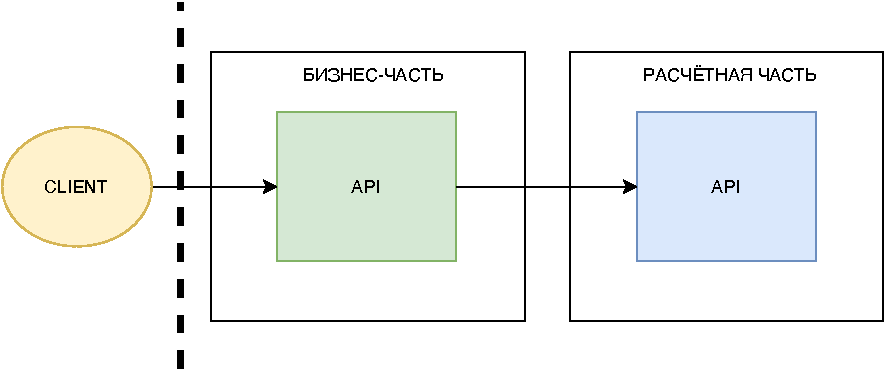
\includegraphics[scale=.9]{pictures/architecture/system}
\end{figure}
\end{frame}

\begin{frame}
\frametitle{Компоненты расчётной части системы}
\begin{figure}
    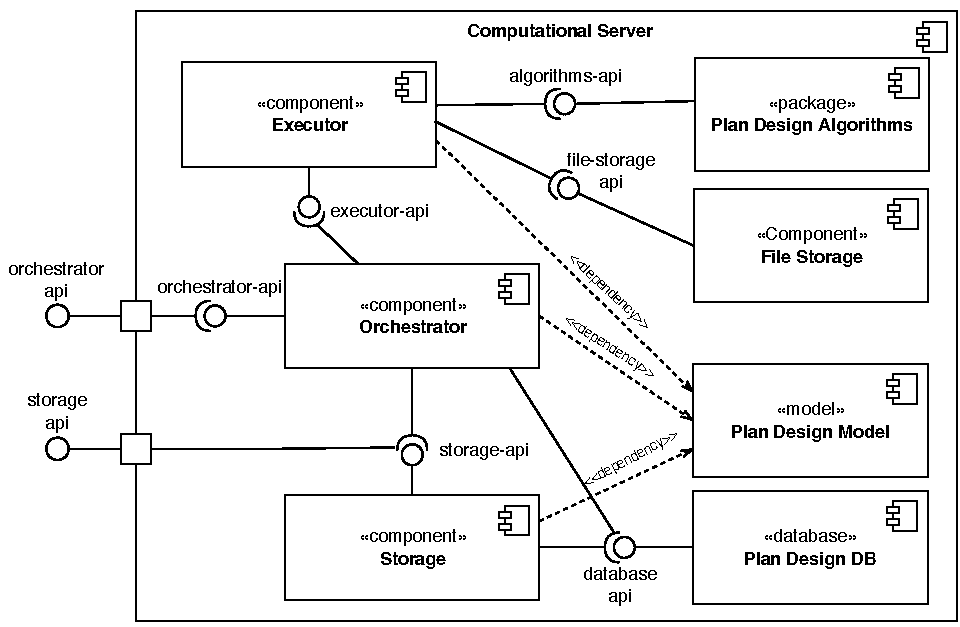
\includegraphics[scale=.67]{pictures/architecture/component}
\end{figure}
\end{frame}

\section{Архитектура данных}

\begin{frame}
\frametitle{Расчётная модель данных}
\begin{figure}
    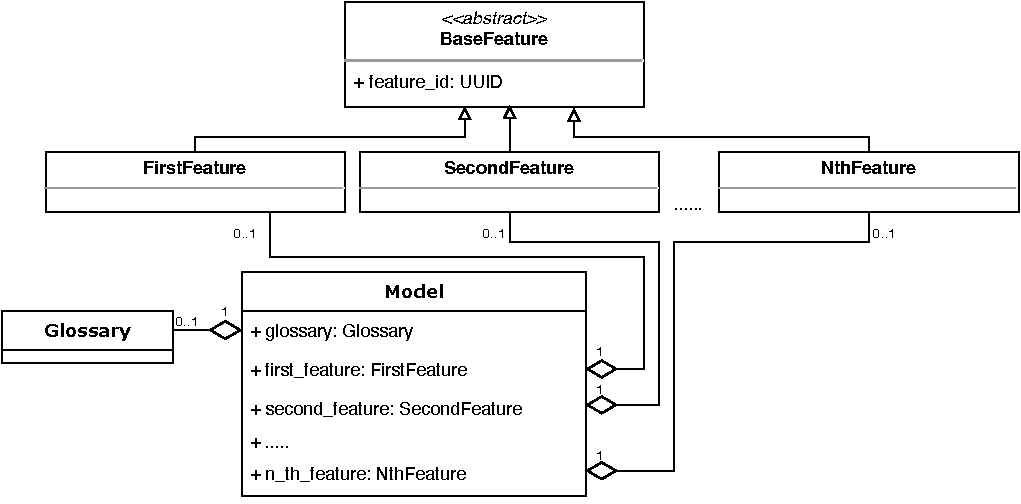
\includegraphics[scale=.7]{pictures/architecture/model_classes}
\end{figure}
\end{frame}

\section{Программная архитектура}

\begin{frame}
\frametitle{Математическая библиотека}
\begin{figure}
    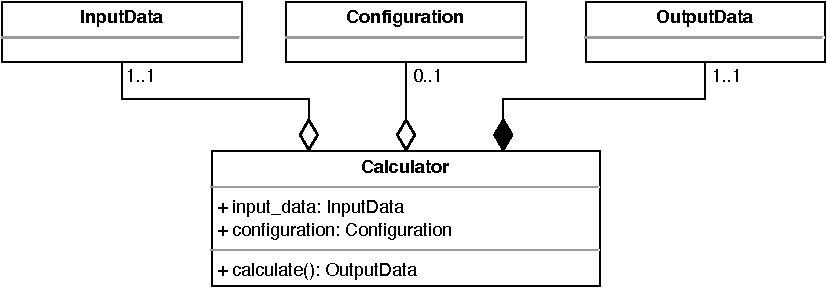
\includegraphics[scale=.9]{pictures/architecture/math_classes}
\end{figure}
\end{frame}

\section{Системная архитектура}

\begin{frame}
\frametitle{Сервис запуска расчётных задач}
\begin{figure}
    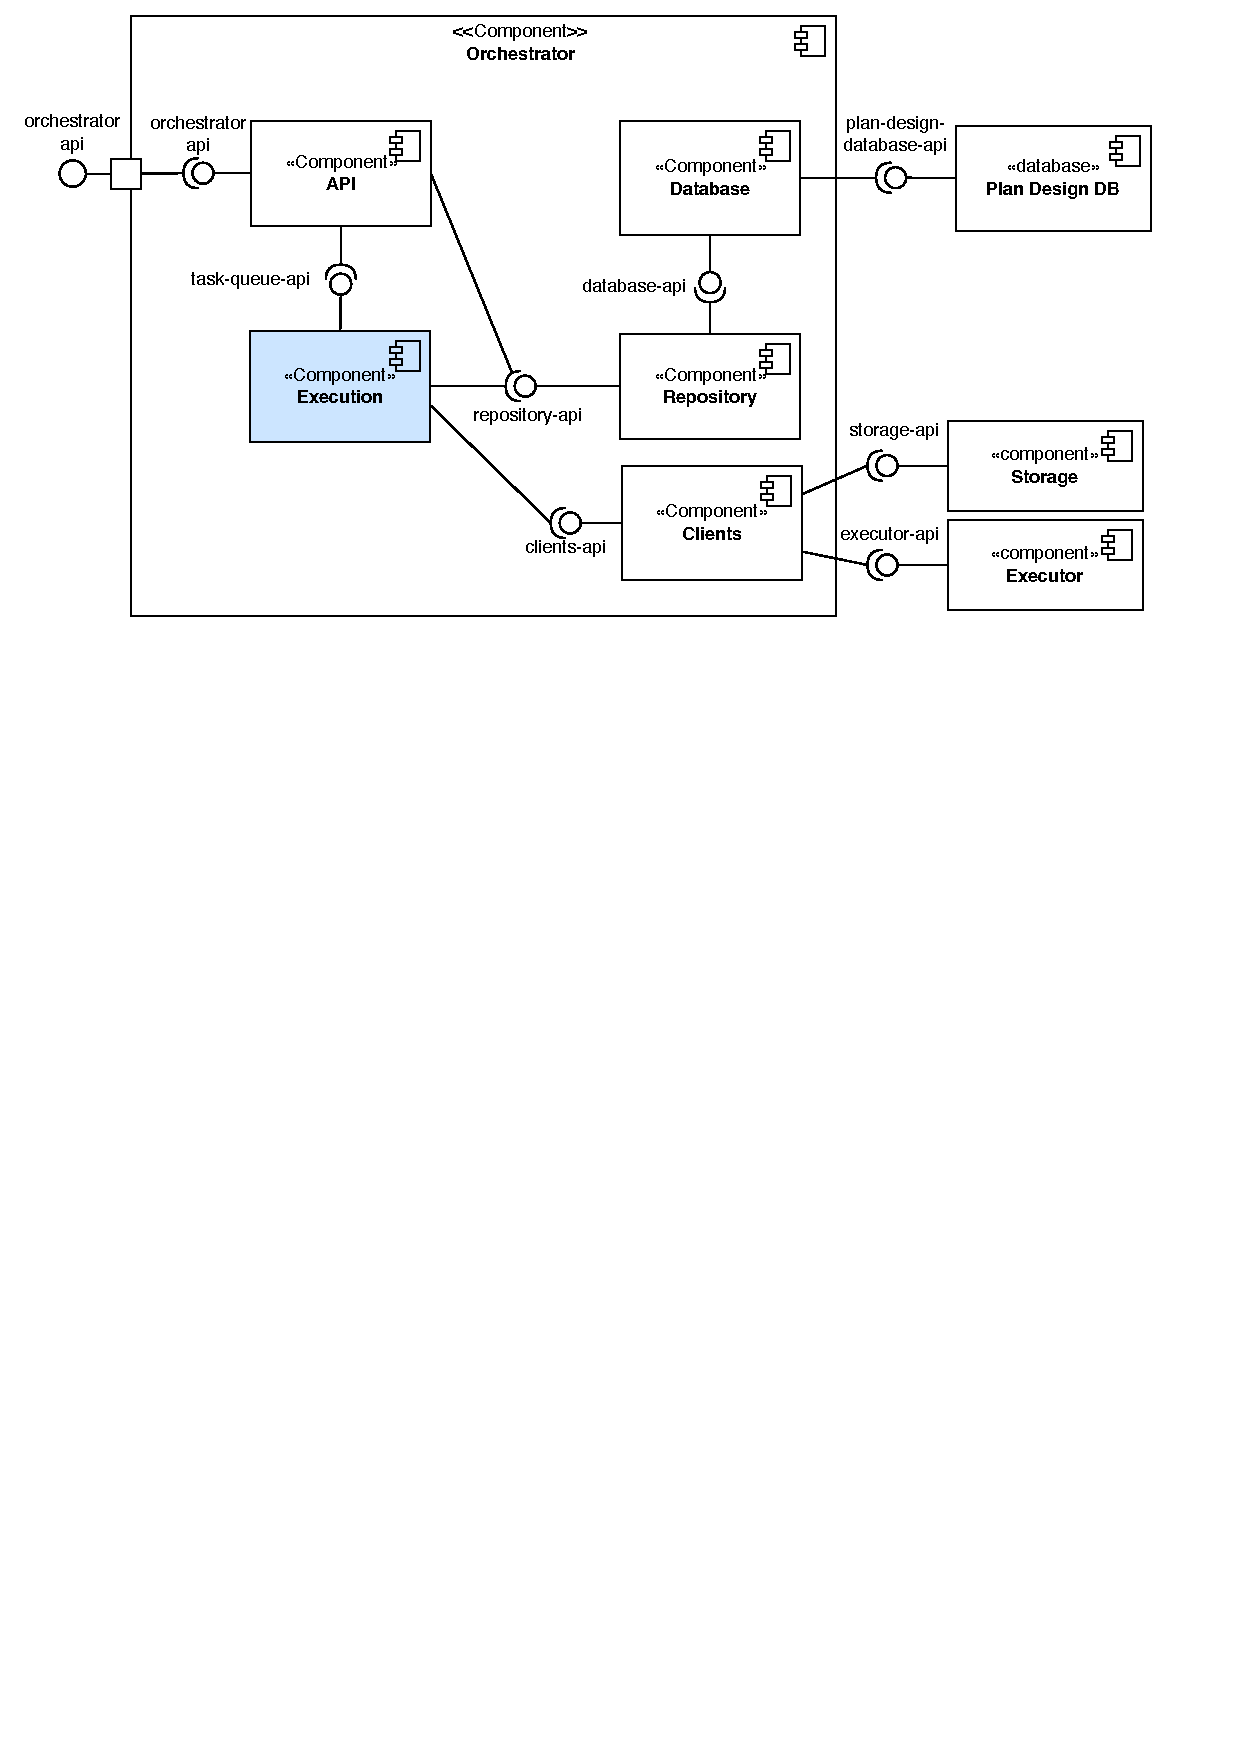
\includegraphics[scale=.6]{pictures/architecture/orchestrator_component_common}
\end{figure}
\end{frame}

\begin{frame}
\frametitle{Диаграмма последовательности запуска расчётных задач}
\begin{figure}
    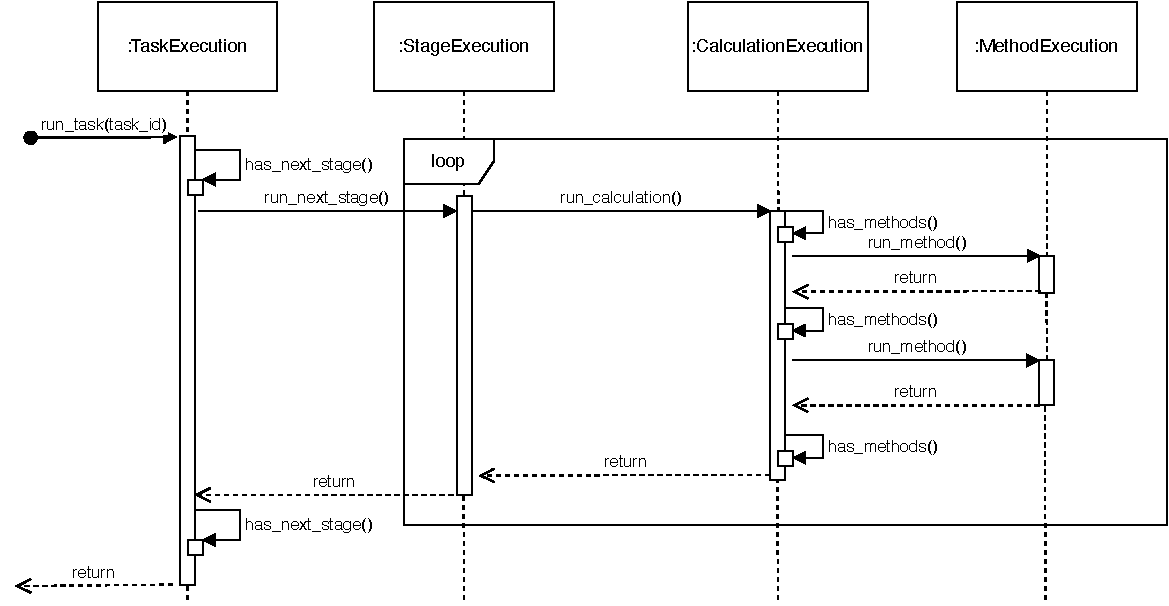
\includegraphics[scale=.7]{pictures/architecture/orchestrator_sequence}
\end{figure}
\end{frame}
